\documentclass{article}
\usepackage{nips10submit_e,times}
%\documentstyle[nips07submit_09,times]{article}
\usepackage[square,numbers]{natbib}
\usepackage{amsmath, epsfig}
\usepackage{amsfonts}
\usepackage{subfigure}
\usepackage{graphicx}
\usepackage{amsfonts}
\usepackage{algorithm}
\usepackage{algorithmic}
\usepackage{easybmat}
\renewcommand\algorithmiccomment[1]{// \textit{#1}}
%
\newcommand{\ignore}[1]{}
\newcommand{\comment}[1]{}
\DeclareMathOperator*{\argmax}{arg\,max}

\title{Probabilistic Deterministic Infinite Automata}


\author{
David Pfau \\
Center for Theoretical Neuroscience \\
Columbia University\\
New York, NY 10027, USA \\
\texttt{pfau@neurotheory.columbia.edu} \\
\AND
Nicholas Bartlett\thanks{ http://www.stat.columbia.edu/~bartlett} \\
Department of Statistics\\
Columbia University\\
New York, NY 10027, USA \\
\texttt{bartlett@stat.columbia.edu} \\`
\And
Frank Wood \\
Department of Statistics\\
Columbia University\\
New York, NY 10027, USA \\
\texttt{fwood@stat.columbia.edu} \\
}

% The \author macro works with any number of authors. There are two commands
% used to separate the names and addresses of multiple authors: \And and \AND.
%
% Using \And between authors leaves it to \LaTeX{} to determine where to break
% the lines. Using \AND forces a linebreak at that point. So, if \LaTeX{}
% puts 3 of 4 authors names on the first line, and the last on the second
% line, try using \AND instead of \And before the third author name.

\newcommand{\fix}{\marginpar{FIX}}
\newcommand{\new}{\marginpar{NEW}}
\newcommand{\q}{\mathsf{q}}
\newcommand{\state}{\mathsf{q}}
\newcommand{\symb}{\mathsf{s}}
\newcommand{\bmu}{\boldsymbol\mu}
\newcommand{\bphi}{\boldsymbol\phi}
\newcommand{\bpi}{\boldsymbol\pi}

%\nipsfinalcopy

\begin{document}

\section{Appendix}
% !TEX root = main.tex
\section{Theory and Related Work}
\label{sec:theory}

The PDIA posterior distribution takes the form of an infinite mixture of PDFAs.  In practice, we run a sampler for some number of iterations and approximate the posterior with a finite mixture of PDFAs.  For this reason, we now consider the expressive power of finite mixtures of PDFAs.  We show that they are strictly more expressive than PDFAs, but strictly less expressive than hidden Markov models.
%
%The natural generalization of PDFAs is to probabilistic {\em non}-deterministic finite automata (PNFA), which are like PDFAs except the transition function $\delta$ is stochastic.  That is, given a state and a symbol emitted from that state, the next state is chosen from distribution over successor states.  \comment{If all successor state distributions assign mass to only one state, the PNFA is a PDFA.}  PNFAs have the same expressive power as hidden Markov models: for any HMM there is a PNFA that defines the same distribution over strings, and vice versa \cite{Dupont2005}.
%
\begin{figure}[htbp]
\begin{center}
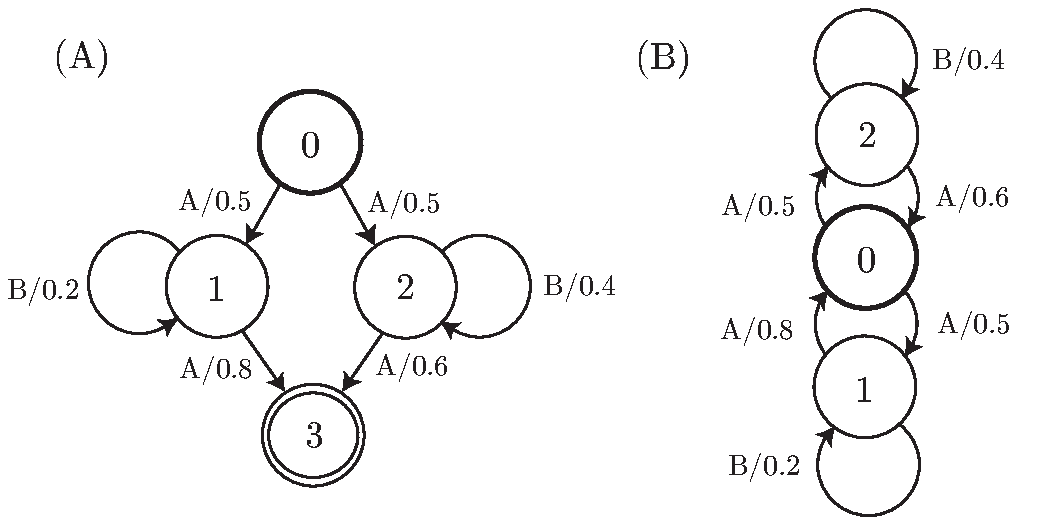
\includegraphics[scale=0.4]{pnfa.pdf}
\caption{Two PNFAs outside the class of PDFAs.  (a) can be represented by a mixture of two PDFAs, one following the right branch from state 0, the other following the left branch.  (b), in contrast, cannot be represented by any finite mixture of PDFAs.}
\label{pnfa}
\end{center}
\end{figure}
%
Probabilistic {\em non}-deterministic finite automata (PNFA) are a strictly larger model class than PDFAs.  For example, the PNFA in \ref{pnfa}(a) cannot be expressed as a PDFA.  However, it can be expressed as a mixture of two PDFAs, one with $Q = \{q_0,q_1,q_3\}$ and the other with $Q = \{q_0,q_2,q_3\}$.  Thus mixtures of PDFAs are a strictly larger model class than PDFAs.  In general, any PNFA where the nondeterministic transitions can only be visited once can be expressed as a mixture of PDFAs.  However, if we replace transitions to $q_3$ with transitions to $q_0$, as in \ref{pnfa}(b), there is no longer any equivalent finite mixture of PDFAs, since the nondeterministic branch from $q_0$ can be visited an arbitrary number of times.    \comment{This can be done by splitting a PNFA with $n$ possible values for $\delta(q_i,s_j)$ into $n$ PNFAs with deterministic $\delta(q_i,s_j)$, and repeating until all transitions are deterministic.  This includes the class of acyclic PNFAs as a trivial subset.  If there are any cycles that return to a state with nondeterministic transition, there is no equivalent finite mixture of PDFAs.}
%
\comment{It is important to note that the algorithm presented here will not always discover the appropriate mixture of PDFAs if the data-generating mechanism is like that in \ref{pnfa}(a).  Our intent is to clarify where the class of models that includes our posterior estimate falls in the Chomsky hierarchy, rather than to make any claim as to what class of models can be efficiently learned.}

Previous work on PDFA induction has focused on accurately discovering model structure when the true generative mechanism is a PDFA.  State merging algorithms do this by starting with the trivial PDFA that only accepts the training data and merging states that pass a similarity test \cite{Carrasco1994,Thollard2000}, and have been proven to identify the correct model in the limit of infinite data.  State splitting algorithms start at the opposite extreme, with the trivial single-state PDFA, and split states that pass a difference test \cite{Ron1996,Shalizi2004}.  These algorithms return only a deterministic estimate, while ours naturally expresses uncertainty about the learned model.

To test if we can learn the generative mechanism given our inductive bias, we trained the PDIA on data from three synthetic grammars: the even process \cite{Shalizi2004}, the Reber grammar \cite{Reber1967} and the Feldman grammar \cite{Feldman1966}, which have up to 7 states and 7 symbols in the alphabet.  In each case the mean number of states discovered by the model approached the correct number as more data was used in training.  Results are presented in Figure~ \ref{fig:synthetic_grammar_and_synth_results}.  Furthermore, the predictive performance of the PDIA was nearly equivalent to the actual data generating mechanism.  Details are given in the appendix.
%
\begin{figure}[htbp]
\centering
\subfigure[Even]{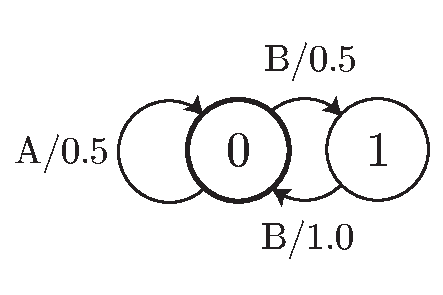
\includegraphics[scale=0.32]{even.pdf}\label{subfig:even}} \hspace{-.55cm} 
\subfigure[Reber]{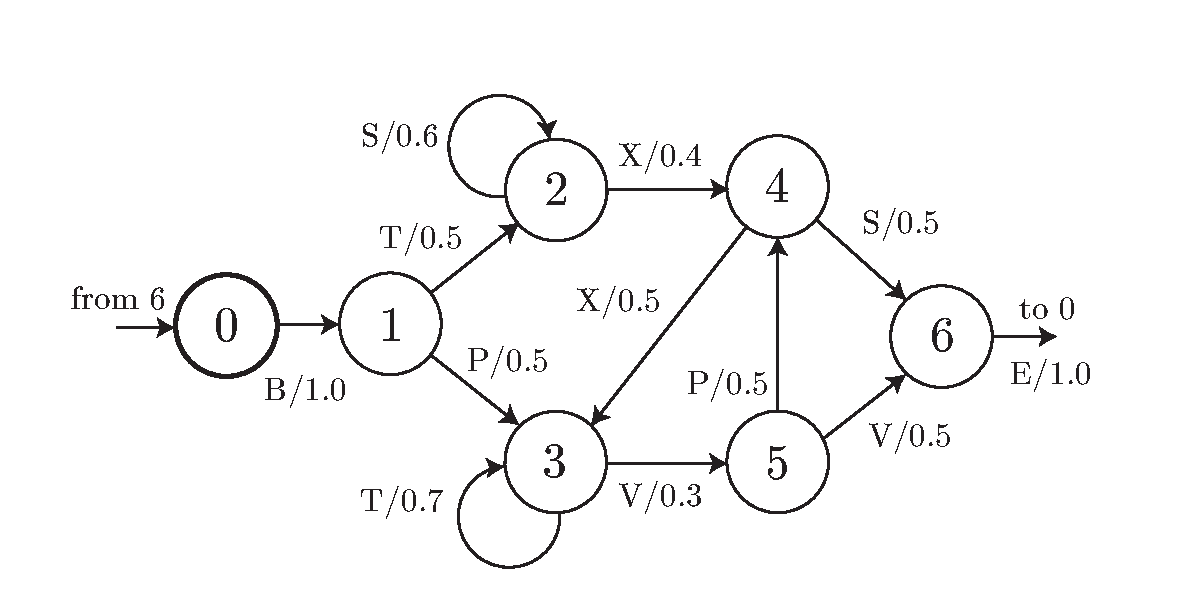
\includegraphics[scale=0.32]{reber.pdf}\label{subfig:reber}}  \hspace{-1.25cm} 
\subfigure[Feldman]{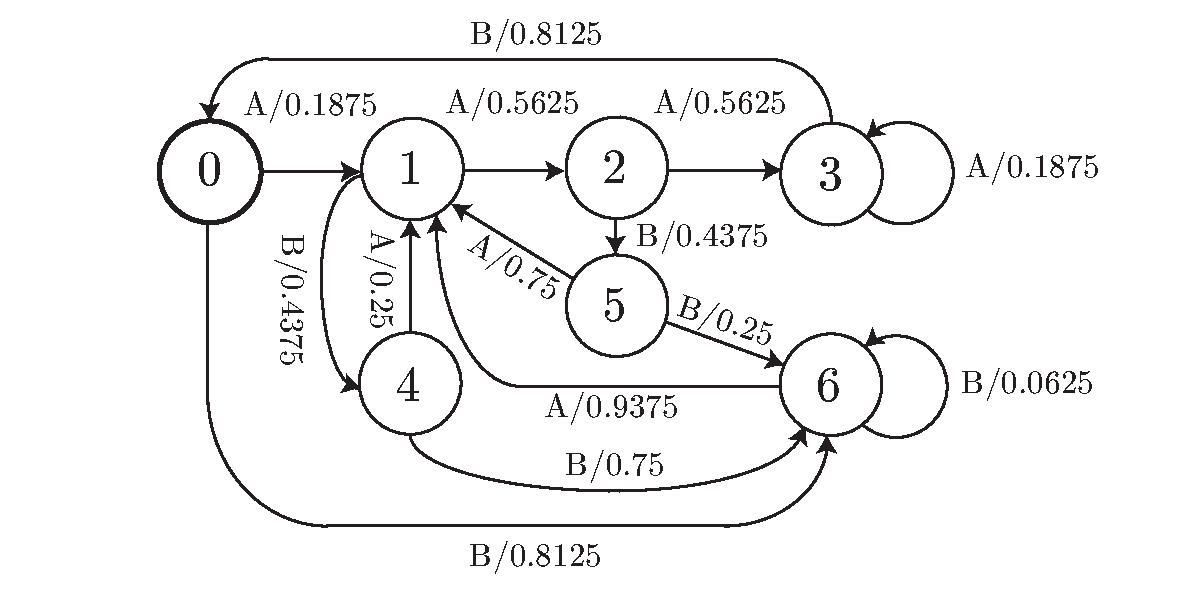
\includegraphics[scale=0.32]{feldman.pdf}\label{subfig:feldman}} \\
\subfigure[Posterior marginal PDIA state cardinality distribution]{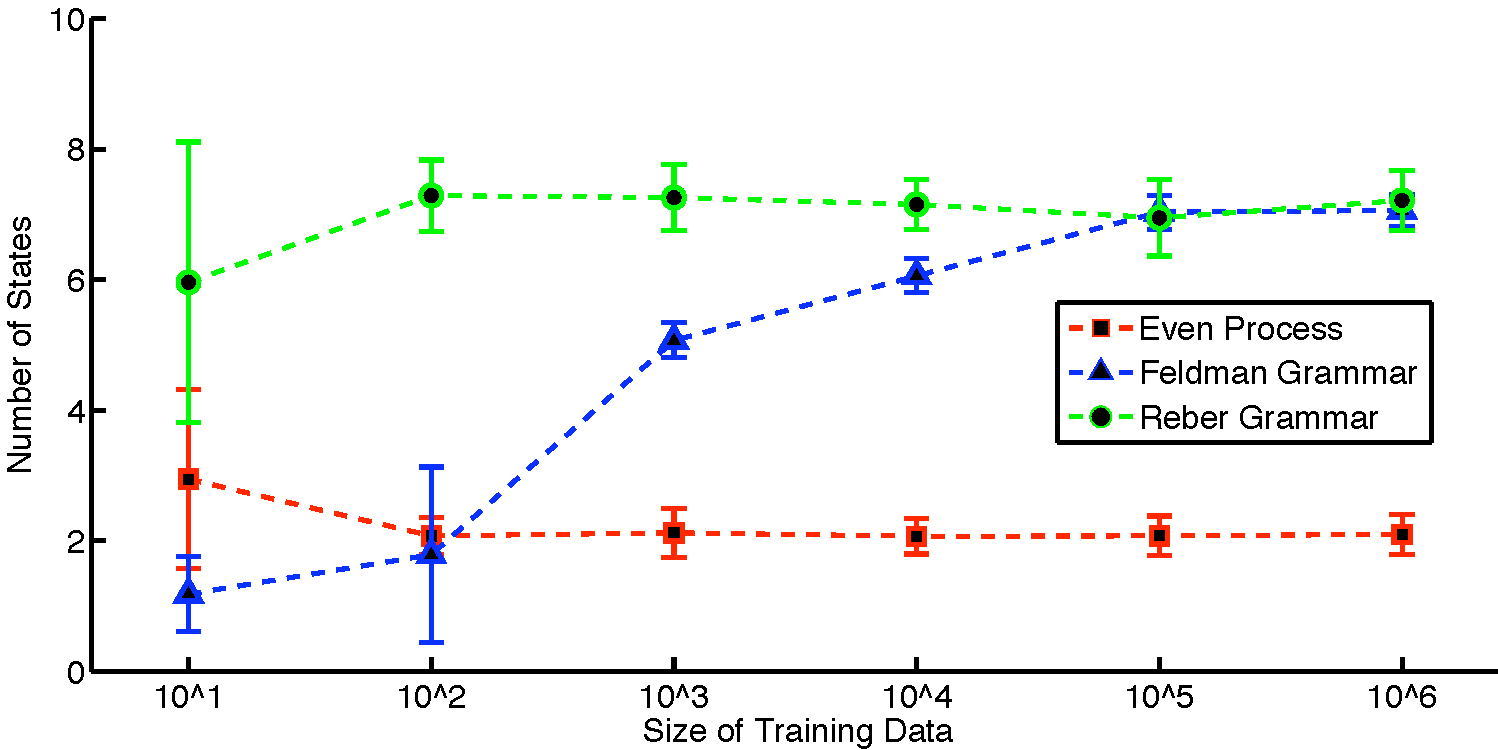
\includegraphics[scale=0.3]{results/syntheticResults.pdf}\label{subfig:posterior}}
\label{fig:synthetic_grammar_and_synth_results}
\caption{Three synthetic PDFAs: \subref{subfig:even} even process, \subref{subfig:reber} Reber grammar, \subref{subfig:feldman} Feldman grammar.  \subref{subfig:posterior} posterior mean and standard deviation of number of states discovered during PDIA inference for varying amounts of data generated by each of the synthetic PDFAs.  PDIA inference discovers PDFAs with the correct number of states}
\end{figure}
\section{Related Work}

Despite a wealth of research on both the theory and practice of learning PDFAs, the work presented here is, to our knowledge, the first algorithm to generate samples from a posterior over automata rather than returning a deterministic estimate.  Prior work has focused on greedy algorithms, which work by either merging or splitting elements of $Q$ according to some statistical test.  Theoretical work has shown that PDFAs are both identifiable in the limit and, with a few restrictions on the model class\footnote{A polynomial number of states in the true automata, a minimum divergence between the distribution over strings that follow two states, and a polynomial bound on the probability of generating strings above a certain length}, are also PAC-learnable\footnote{A model class is said to be {\em PAC-learnable} if there is an algorithm that will return, in time polynomial in $\frac{1}{\delta}$,$\frac{1}{\epsilon}$ and $|D|$, an estimate within an accuracy $\epsilon$ of the true model from $|D|$ examples with probability $1-\delta$.} using KL divergence between automata as a measure of accuracy.

\subsection{State Merging Algorithms}
A variety of algorithms work by starting with the trivial automata built from the prefix tree of the data, and generalizes by merging states that pass a similarity test.  Merging two states is not trivial: if $\delta(q_1,s_j) \ne \delta(q_2,s_j)$, then merging $q_1$ and $q_2$ will produce a state with nondeterministic transitions.  This is avoided by recursively merging the states $\delta_{1j}$ and $\delta_{2j}$ until the resulting automata is deterministic.  The result is a {\em quotient automata} of the original.  One of the earliest algorithms to use this method is ALERGIA \cite{Oncina1994}, which uses a test based on the Hoeffding bound to decide whether to merge states, and was proven to converge to the true automata in the limit of infinite data.

Later algorithms have mostly focused on improving the state merging test.  MDI uses a test based on the KL divergence between automata, and penalizes automata with many states.  Thus it can be interpreted as a greedy maximum posterior estimator with a minimum description length prior.  Empirically, it has better predictive performance than ALERGIA on natural language data.

\cite{Clark2004} presented a state-merging algorithm for cyclic PDFAs that is PAC-learnable given very few restrictions on the model class.  While the emphasis was on theoretical rather than empirical performance, it was also shown to work well from small data.

\subsection{State Splitting Algorithms}

State splitting algorithms, by contrast, start with the most general single-state automata and become more selective by adding more states.  \cite{Ron1995} learned a variable-order Markov model using a state-splitting algorithm, where a state corresponding to a string suffix was split into states corresponding to longer suffixes according to some test (*hm...all this "according to some test" is getting redundant.  Might want to rephrase this*).  Splitting might occasionally produce nondeterministic transitions.  For example, after splitting the context $01$ into $001$ and $101$, the context $0$ and symbol $1$ might transition to either one, unless the context $0$ is also split into $10$ and $00$, but these probabilistic suffix trees could be mapped onto PDFAs after learning.

CSSR \cite{Shalizi2004} took a similar approach, but with a model class that contains all PDFAs.  Their philosophical motivation, similar to ours, is to learn the minimal sufficient statistics for predicting the future given the past.  Given a stationary sequence with infinitely long past and future, those statistics form a PDFA, which they call a {\em causal state machine}.  Each state is a set of suffixes, rather than a single suffix, which means the model class includes all PDFAs.  If the predictive distribution for a suffix passes a Kolmogorov-Smirnov test, that state is split in two and suffixes in the original state are divided.  Nondeterministic transitions are removed recursively by backing up to the states preceding a split state and splitting in the natural way, much like the reverse of how states are merged when forming quotient automata.

\end{document}
